\chapter{Referencial Teórico}

% Falar sobre RSL

Visando obter uma revisão de literatura eficaz foi feita uma Revisão Sistemática de Literatura, com base no relatório técnico de \cite{Kitchenham}. Diante disso, o projeto se torna mais abrangente do ponto de vista de pesquisa literária e ao mesmo tempo mais restritivo, realmente realizando o estudo dos objetos que são importantes para a pesquisa e seus resultados.

% Bases pesquisadas

Como o objetivo do trabalho tem foco na resultado prático, geralmente as bases relacionadas às áreas mais técnicas, como Ciência da Computação, devem ser bem focadas, como IEEE e ACM, por exemplo. Outras bases de natureza mais genérica também foram pesquisadas, geralmente através do site da CAPES, mas com caráter mais de apoio teórico realmente.

Embora a amplitude desta área de estudo, alguns detalhes necessitam ser observados para evitar assim redundância e perda de foco. A pesquisa necessitava ser focada em técnicas de extração de metadados em artigos científicos, somente. Estas técnicas necessitam ser reais, de maneira a existir realmente uma forma prática de serem testadas, fazendo assim com que os resultados obtidos sejam comparados e confrontados para verificar então a eficácia deste processo.

Como a pesquisa necessita de um resultado prático eficaz os critérios que serão adotados para demonstrar a relevância de um estudo serão seus resultados. Com base em uma técnica potencialmente eficaz, esta deve ser testada juntamente com um grupo de artigos previamente selecionados. Estes artigos já possuirão seus dados mapeados de maneira a poder comparar os resultados obtidos com cada uma das técnicas e seus respectivos resultados. Portanto os critérios utilizados serão de natureza explicitamente prática, com foco em resultados concretos, numericamente representados.

% Falar sobre os eventos encontrados na área

Seguindo as orientações propostas em \cite{Kitchenham} foram mapeados alguns eventos para serem pesquisados, a fim de encontrar trabalhos relevantes para a área. Sendo assim, foram mapeados os seguintes eventos:

\begin{itemize}
\item KDIR (International Conference of Knowledge Discovery and Information Retrieval)
\item ICDAR (International Conference on Document Analysis and Recognition)
\item PDCAT (International Conference on Parallel and Distributed Computing, Applications and Technologies)
\item IAPR (International Workshop on Document Analysis Systems)
\item ACM Conference on Digital Libraries
\end{itemize}

\begin{textoalterado}
Estes eventos foram analisados, observando todas as citações e referências utilizadas, a fim de encontrar também detalhes importantes para a pesquisa, sem perder o foco do trabalho.
\end{textoalterado}

\section{Metadados}

\comentario{Esta nova seção foi incluída para definir alguns conceitos que são apresentados mais a frente com a apresentação das técnicas.}

\subsection{Conceito de Metadado}

\begin{textonovo}

Com base nas ideias apresentadas por \cite{meta-dados}, podemos definir inicialmente um metadado da seguinte maneira:

\begin{quote}
\textit{''[...] an element of metadata describes an information resource, or helps provide access to an information resource.''}
\end{quote}

Sobre este aspecto conclui-se que todo dado que agregue nova informação a um recurso pode ser considerado um metadado. Desta maneira, quanto mais metadados um recurso tiver, mais detalhado ele é, ou seja, mais dados sobre ele temos. Com efeito, podemos simplificar ainda mais a definição de metadado com sendo \textit{um conjunto de dados sobre um determinado recurso}.

Temos contato diariamente com diversos metadados, sejam eles visíveis naturalmente ou não, mas de uma maneira ou outra, são utilizados em tarefas do cotidiano de maneira ampla; geralmente um conjunto enorme de novos dados e informações sobre recursos dos mais diversos tipos e modelos.

Podemos citar, por exemplo, a utilização de pequenos pedaços de dados sobre um conjunto de livros, dentro de um ambiente de biblioteca, por exemplo, o que é considerado uma coleção de elementos de metadados, conforme pode ser confirmado em \cite{meta-dados}. Além disso, o mesmo autor cita como exemplos de metadados os dados coletados por mecanismos de busca no momento em que as páginas da Internet são indexadas e então armazenadas.

Ante o exposto, podemos criar e identificar diversos conceitos do que podemos chamar de metadado, porém, em virtude de sua enorme aplicação e significância, alguns detalhes dentro do escopo deste trabalho devem ser direcionados, visando identificar e explicar melhor os conceitos que serão aplicados na análise das ferramentas e técnicas que aqui serão apresentadas.

\end{textonovo}

\subsection{Padrões de Metadados}
\label{padroes-de-metadados}

\begin{textonovo}

Diante da infinidade de dados que podem estar atrelados a um recurso, temos uma amplitude muito grande de características que podem ser definidas como sendo metadado. Por isso, foram definidos 15 (quinze) elementos de metadados para descreverem um recurso informacional, independente da disciplina em questão, estabelecendo então um padrão. 

Para isso, foi criado o padrão Dublin Core \cite{dublin-core}, que se originou após uma série de encontros feitos desde 1995, unindo bibliotecários e pesquisadores digitais e de conteúdo, visando identificar padrões para se representar um recurso eletrônico, seja ele uma página, um texto ou até mesmo um documento em um determinado formato. O nome ''Dublin'' foi dado em virtude da primeira reunião do grupo, que foi realizada em Dublin, Ohio. Já o nome ''core'' se deu em virtude dos elementos serem amplos e genéricos, sendo então utilizados para descrever uma grande variedade de recursos.

Os quinze elementos que fazem parte do padrão Dublin Core compartilham de um vasto conjunto de vocabulários de metadados, juntamente com diversas especificações técnicas, que são mantidas pela Dublin Core Metadata Initiative (DCMI), a agência responsável pela definição destes elementos.

Este padrão é utilizado nos dias atuais para se representar um recurso na Internet, por exemplo, podendo ser qualquer coisa que possa ser identificada \cite{dublin-core-1-1}. Com base em suas características, mecanismos de busca podem indexar um recurso de maneira mais rápida e precisa, pois este é acompanhado de pequenas sinalizações sobre seu conteúdo, que são os metadados. 

Para cada elemento descrito pelo padrão temos informações como: 

\begin{itemize}
\item \textit{label}, que é o texto para leitura e entendimento humano;
\item \textit{name}, que é usado para o processamento de máquina, ou seja, um identificador que a máquina utiliza para reconhecimento.
\end{itemize}

Os elementos que fazem parte da versão 1.1 do padrão Dublin Core \cite{dublin-core-1-1} podem ser vistos no \refanexo{anexo-dublin-core} deste trabalho.

Abaixo podemos ver um exemplo de código para utilização de metadados Dublin Core em uma página da Internet, por exemplo, onde iremos referenciar os elementos \textit{creator}, \textit{title} e \textit{language}.

\lstset{language=HTML}
\begin{lstlisting}[escapechar=\#]
<meta name="DC.Creator" content="Junior Grossi" >
<meta name="DC.Title" content="#\imprimirtitulo#" >
<meta name="DC.Language" content="pt_BR" >
\end{lstlisting}

Desta forma, a indexação do autor (\textit{DC.Creator}) da página, bem como seu título (\textit{DC.Title}) e idioma (\textit{DC.Language}), são feitos de maneira bem simplificada e direta. Para páginas da Internet, com as informações todas em formato HTML, a utilização destes metadados perderiam o sentido, visto que essas informações poderiam ser facilmente encontradas de outras formas, como a análise do próprio código HTML. Porém, para documentos binários - em formato PDF ou Word, por exemplo - a utilização destes metadados é de suma importância, visto que permite que essas informações básicas sejam capturadas sem a necessidade de análise do conteúdo dos arquivos, o que traria complexidade ao processo.

\end{textonovo}

\subsection{Técnicas de Extração de Metadados}

Algumas técnicas e algoritmos de extração de metadados são utilizadas em diversos projetos, de maneira a serem citadas em momentos onde exige-se uma precisão maior.

Estas técnicas se baseiam basicamente na classificação de dados com base nas suas representações escritas, tanto baseadas em padrões preestabelecidos ou até mesmo com base em um dicionário de palavras capaz de reconhecer ocorrências em diversas partes de um documento, o que agrega assertividade ao processo de extração.

\subsubsection{Support Vector Machines (SVM)}
\label{tecnica-svm}

\begin{textonovo}
Support Vector Machines (SVM) é uma técnica de \textit{machine learning} que permite que um conjunto de dados sejam analisados, possibilitando que padrões sejam extraídos, criando uma espécie de memória \cite{Vapnik-SVM}. Seu objetivo inicial era ser uma técnica de classificação de dados, por ser focada em reconhecimento de padrão através de análises matemáticas.

Esta técnica se baseia na redução de erros com base em um resultado de treinos consecutivos que permitem a criação de um padrão e estabelecem um aprendizado por parte da distância entre ocorrências \cite{Vapnik-SVM}. Todas as análises realizadas são mapeadas, permitindo que um registro histórico em forma matemática seja realizado, levando o algoritmo à possibilidade de diferenciação entre um resultado e outro, de forma numérica.

De acordo com Chieu \cite{Chieu}, ele sugere que a tarefa de extrair informação pode ser considerada um problema de classificação. Partindo deste pensamento foi que Han \cite{Han-SVM} decidiu utilizar técnicas de SVM para extração de metadados, utilizando das qualidades matemáticas do processo no reconhecimento de padrões, o que permitiu que novas descobertas fossem feitas, expandindo o estudo da extração de dados para um patamar mais amplo e elevado.

\end{textonovo}

\begin{textoalterado}
Várias ferramentas de extração se baseiam na utilização de SVM como técnica principal, visto sua eficiência no reconhecimento de padrões. Como descrito por \cite{Han-SVM} a utilização desta técnica é baseada na identificação de campos previamente selecionados no cabeçalho de um documento, do qual se deseja obter os metadados, por exemplo.

Esta técnica analisa diversos campos chamando-os de classes, e atribui a cada classe uma característica que a permite ser identificada. Deste modo, cada linha do cabeçalho do documento é classificada em uma ou mais classes, onde algumas fazem parte do padrão Dublin Core, detalhado na \autoref{padroes-de-metadados}.

Seymore et al. \cite{Seymore-HMM-IE} definiu 15 (quinze) \textit{tags} para esta definição do cabeçalho de um documento. Porém, destas 15 (quinze) \textit{tags} definidas, somente 4 (quatro) correspondem ao padrão da Dublin Core e estão ilustradas na \autoref{tab:svm-classes}. Estas também foram as \textit{tags} utilizadas por Han para a extração de metadados dos cabeçalhos de artigos científicos \cite{Han-SVM}.

\end{textoalterado}

\begin{table}
    \caption{Relação de classes utilizadas e comparação com o padrão Dublin Core.}
    \begin{center}
        \begin{tabular}{|C{3cm}|C{3cm}|p{7cm}|}
            \hline \textbf{Classe (Tag)} & \textbf{Referência Dublin Core} & \textbf{Descrição}\\ 
            \hline Title & Title & Título do artigo\\
            \hline Author & Creator & Nome do autor do documento\\
            \hline Affiliation & & Afiliação do autor\\
            \hline Address & & Endereço do autor\\
            \hline Note & & Frases de reconhecimentos, \textit{copyright}\\
            \hline Email & & Endereço de e-mail do autor\\
            \hline Date & & Data da publicação\\
            \hline Abstract Introdution & Description & A parte de introdução do artigo\\
            \hline Phone & & Telefone do autor\\
            \hline Keyword & Subject & As palavras-chave do documento\\
            \hline Web & & Endereço na Internet do autor\\
            \hline Degree & & Associação com o grau acadêmico\\
            \hline Pubnum & & Número da publicação do documento\\
            \hline Page & & O final da página\\
            \hline
        \end{tabular}
    \end{center}
    \label{tab:svm-classes}
\end{table}

\begin{textonovo}
A ocorrência dos campos é mapeada em uma representação bidimensional, permitindo identificar visualmente os padrões encontrados na análise de cada classe. Desta forma, com a visualização do posicionamento de cada ocorrência é possível obter uma distância clara entre os pontos de reconhecimento, chamada pelo autor de \textit{hyperplanes} \cite{Vapnik-SVM}. Por sua vez, estes pontos são marcados como sendo os ''support vectors'', que permitem que o \textit{hyperplane} entre eles determine a divisão entre as classes de forma clara e eficaz, como pode ser visto na \autoref{fig:svm-grafico}. Esta divisão permite então a distinção entre os metadados, diferenciando os elementos analisados pelo algoritmo.
\end{textonovo}

\begin{figure}
	\centering
	\caption{Distância representando a separação entre classes na técnica de SVM.}
	\label{fig:svm-grafico}
	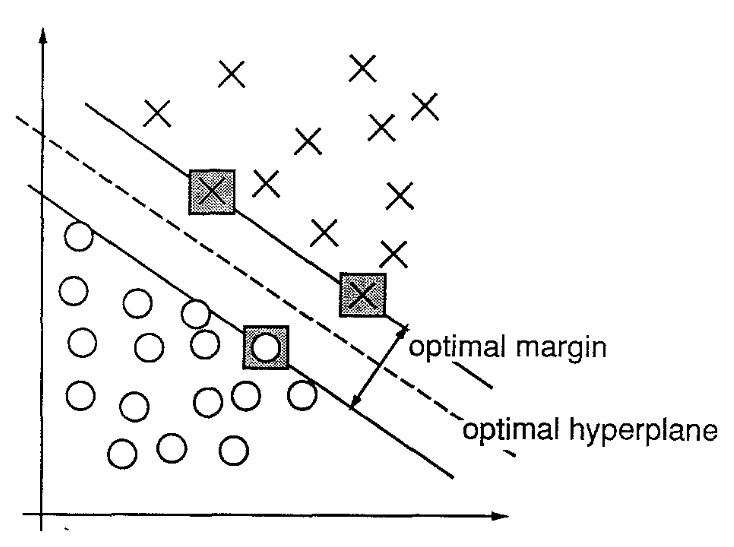
\includegraphics[width=0.6\linewidth]{./assets/svm-grafico}
\end{figure}

\begin{textoalterado}
Além desta análise são utilizadas comparações de palavras dentro de um contexto previamente selecionado. Assim foi criado um \textit{cluster} de palavras comuns que facilita na identificação destas classes nos cabeçalhos analisados. Este \textit{cluster} basicamente é composto de:
\end{textoalterado}

\begin{itemize}
\item Dicionário online padrão em sistemas Linux;
\item 8441 nomes e 19613 sobrenomes;
\item Sobrenomes chineses;
\item Nome dos estados do Estados Unidos e das províncias canadenses;
\item Nomes das cidades dos Estados Unidos;
\item Nome dos países do mundo, de acordo com World Fact Book\footnote{Disponível em \url{https://www.cia.gov/library/publications/the-world-factbook/index.html}};
\item Nome dos meses e suas respectivas abreviações.
\end{itemize}

Para cada uma das classes analisadas são feitas correlações com o tipo de dado esperado, de maneira a permitir que endereços de e-mail, por exemplo, sejam extraídos com base em expressões regulares utilizadas em linguagens de programação.

\begin{textonovo}
Support Vector Machine é uma técnica conhecida principalmente por sua boa performance e habilidade para com grandes quantidades de dados, sendo por isso considerada uma boa solução para problemas de classificação. Por essa característica sua principal funcionalidade é baseada em opções, e a que mais se assemelha com a análise realizada é então classificada. Por isso Han \cite{Han-SVM} decidiu utilizar este mesmo conceito de comparação para ser então aplicado na extração de dados, de modo a confrontar e comparar classes de metadados, a fim de identificá-los e diferenciá-los.

Han também encontrou alguns desafios na diferenciação de campos, como é o caso dos múltiplos autores. Em alguns casos a diferenciação de autores, que fazem do mesmo campo, poderiam estar até em linhas ou grupos diferentes. Para isso foram utilizados alguns elementos para representar a separação dos nomes (\textit{chunks}), como pontuações e a palavra ''and''. Desta forma, os autores eram extraídos seguindo este padrão estipulado.

O resultado obtido pela utilização de SVM como técnica de extração de metadados foi bem relevante. O autor realizou uma comparação com a aplicação da técnica de Hidden Markov Models (HMM) - detalhada na \autoref{tecnica-hmm} - onde a SVM se mostrou mais eficaz na precisão da extração para algumas classes específicas, como é o caso dos títulos, autores e endereços, por exemplo. Para outras classes a utilização da técnica de HMM ainda demonstrou ser mais eficiente na extração de metadados.

\end{textonovo}

% Han também utiliza dicionários para facilitar na extração das informações

%Para o caso de extração de metadados em artigos científicos utilizando \textit{Support Vector Machines} \cite{Han-SVM} as tags de Seymore et al. \cite{Seymore-HMM-IE} são utilizadas para representação destas classes.

%Deste modo, com base nestas classes são definidas características de suas classes vizinhas, como por exemplo, elementos que ficam perto de outros elementos, que possuem uma sequência lógica geral de exibição. Com base nestas informações, que são feita classe por classe, estes padrões vão sendo encaixados a cada linha do cabeçalho analisado, permitindo que os metadados sejam extraídos com uma grande precisão.

% % % % % % % % % % % % % % % % % % % % % % % % % % % % % % % %
% % % % % Parei a revisão aqui em 17/03/2015 23:22 % % % % % % % % %
% % % % % % % % % % % % % % % % % % % % % % % % % % % % % % % %

\subsection{Hidden Markov Models (HMM)}
\label{tecnica-hmm}

A teoria básica de Markov foi conhecida próximo dos anos 80 por engenheiros e matemáticos com grande aplicação inicialmente em processamento da fala, mas com vasta amplitude em outras áreas onde a descoberta de padrões pode ser aplicada \cite{Rabiner-HMM}.

O processo é baseado na identificação de modelos observáveis que representem e caracterizem a ocorrências de símbolos, ou seja, padrões, em determinados estados. Se um sinal foi observado ele pode ser utilizado para futuras referências, de acordo com o padrão. 

Um exemplo prático citado por Rabiner e Juang \cite{Rabiner-HMM} é o caso de uso do jogo  \textit{Cara e Coroa}. Toma-se um observador em um quarto fechado com uma cortina totalmente fechada para outro cômodo. Este observador não consegue ver nada que acontece no outro cômodo, onde está uma outra pessoa jogando uma moeda pra cima, relatando sempre o resultado obtido (cara ou coroa). Neste caso o problema é construir um modelo Hidden Markov Model (HMM) para explicar ao observador a sequência dos resultados obtidos. 

Neste exemplo, o primeiro caso é baseado tanto no estado de cada resultado (cara ou coroa) e em probabilidades matemáticas de ocorrência destes estados, neste caso, 0.5, ou seja, dois estados. Assim desenha-se modelos onde os estados são representados com base nas inúmeras possibilidades existentes, levando inclusive em consideração a sequência dos últimos acontecimentos. \begin{textonovo}Outra possibilidade seria a existência de duas moedas, o que daria ainda dois estados existentes, mas não em função da probabilidade de sair cara ou coroa, mas sim por serem consideradas duas moedas ''justas'', o que daria também uma probabilidade de 0.5 pra cada.

Neste último exemplo o grande detalhe do modelo é que este é oculto (\textit{hidden}). Isso se deve ao fato de os dois estados, representados pelas duas moedas, serem totalmente independentes, o que não permite identificar qual moeda é a ''justa'' e então informar ao observador o resultado daquela rodada.

Por esta alteração de resultados e probabilidades, o fator decisivo na criação de cada modelo é a definição do número de estados que ele terá. Além disso, outro ponto que determina o sucesso do método é a utilização de um resultado anterior - \textit{training data set} -, ou seja, uma memória, um conjunto de informações pré-identificadas que permitiriam ainda à associação dos estados e ocorrência dos símbolos \cite{Rabiner-HMM}.

Um HMM pode ser formado por um conjunto de elementos, que formarão toda a teoria e aplicação dos algoritmos dentro do processo:

\begin{enumerate}
\item Um número \texttt{N} de estados, onde \texttt{N} é um inteiro finito;
\item Um intervalo temporal \texttt{t}, que determina a entrada em um novo estado, através de uma transição de probabilidade entre eles, levando em consideração sempre o estado anterior;
\item Após cada transição o observador registra um \texttt{símbolo} de acordo com a distribuição de probabilidade, que por sua vez depende do estado atual do modelo.
\end{enumerate}

A utilização dos resultados passados - \textit{training data set} - é muito importante para uma boa definição de um HMM, visto que permite adaptar os parâmetros do modelo para aquele conjunto de dados passados, que por sua vez fazem parte de um padrão já identificado.

Seguindo este padrão o HMM pode ser utilizado, por exemplo, para reconhecimento de palavras isoladas que, juntamente com a utilização de um vocabulário de palavras permite a criação de modelos de reconhecimento. Cada palavra deste vocabulário seria um modelo HMM, permitindo que a palavra escolhida fosse a pertencente ao modelo com maior probabilidade.

\end{textonovo}

Já no âmbito da extração da informação, o HMM pode ser aplicado conforme é apresentado por Seymore et al. \cite{Seymore-HMM-IE}, onde um modelo construído manualmente contendo múltiplos estados por campos (título, autor, etc), pode ser mais eficiente do que um modelo com um estado por campo. 


\begin{figure}
\centering
\caption{Exemplo de modelo HMM, onde X são os estados, Y as observações possíveis, A as probabilidades de mudança de estado e B as saídas das probabilidades.}
\label{fig:hmm-states}
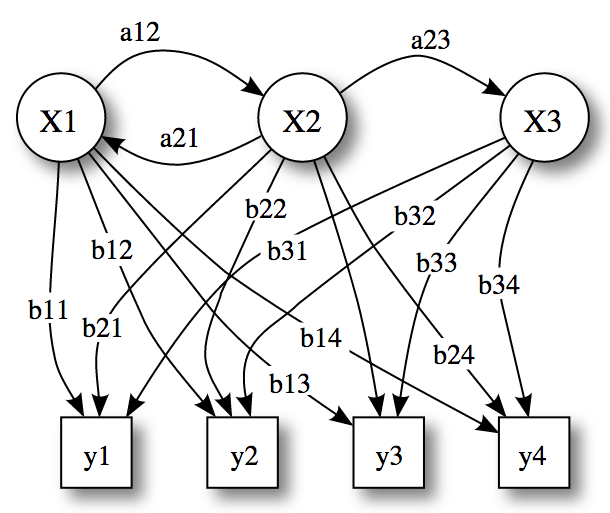
\includegraphics[width=0.7\linewidth]{./assets/hmm-states}
\end{figure}

\begin{textoalterado}
Um dos pontos positivos deste modelo é que por serem baseados em estatística eles são muito bem empregados em problemas de linguagem natural, aliando os resultados positivos à excelente performance computacional. Como desvantagem deste método podemos citar o fato de, por ser baseado em estatística, uma grande quantidade prévia de dados deve ser utilizada a título de treino para se obter padrões significativos para então ser aplicados de maneira final na criação do modelo.
\end{textoalterado}

Deste modo, para extração dos metadados, o HMM pode ser utilizado aplicando um marcador (\textit{label}) em cada palavra do cabeçalho de um documento (artigo científico), relacionando cada palavra a uma classe, como título, autor, etc. \begin{textonovo}Assim, uma opção seria a criação de um modelo com \texttt{N} estados, onde cada estado corresponderia a uma classe que se deseja extrair - por exemplo o título do documento. Porém, no caso da existência de sequências ocultas (\textit{hidden sequences}) - o que alteraria a seleção do estado seguinte - a utilização de vários estados para cada classe traria resultados melhores \cite{Seymore-HMM-IE}.

% % % % % % % % % % % % % % % % % % % % % %
% % % % % % % % % % % % % % % % % % % % % %
% % Terminar de falar do Seymore-HMM-IE
% % % % % % % % % % % % % % % % % % % % % %
% % % % % % % % % % % % % % % % % % % % % %

Uma outra utilização de HMM na extração de informação é descrita por \cite{Zhang-HMM-IE}, onde é realizado um experimento de extração de informação utilizando um conjunto de dados semi-estruturados em formato HTML contendo informações sobre restaurantes da cidade de Los Angeles.

Neste caso são estipulados quatro estados para o modelo: \textit{Background}, \textit{Prefix}, \textit{Suffix} e \textit{Target}. O \textit{Target} é o estado responsável pela emissão do símbolo - chamado pelo autor de \textit{token} - para o ''campo-alvo''. O \textit{Preffix} e \textit{Suffix} são estados que emitem símbolos que aparecem respectivamente antes e depois deste campo-alvo. Todos os demais símbolos são emitidos no estado \textit{Background}. A relação entre os estados pode ser visualizada na \autoref{fig:zhang-hmm-ie}.

\begin{figure}
	\centering
	\caption{Estados utilizados por \cite{Zhang-HMM-IE} em seu modelo HMM.}
	\label{fig:zhang-hmm-ie}
	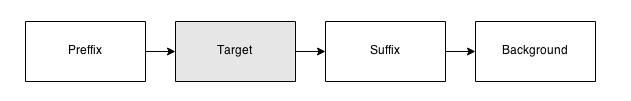
\includegraphics[width=0.8\linewidth]{./assets/zhang-hmm-ie}
\end{figure}

Os seguintes campos deveriam ser extraídos das informações dos restaurantes: \textit{restaurant name} (nome do restaurante), \textit{telephone number} (número de telefone), \textit{hours (horas)} e \textit{cuisine} (tipo de comida servida, como italiana, alemã, etc). Segundo Zhang \cite{Zhang-HMM-IE} os campos \textit{restaurant name} e \textit{telephone number} deveriam ser mais fáceis de serem obtidos, visto que o nome do restaurante geralmente se encontra em destaque, com alguma diferenciação visual. Já o telefone possui um padrão numérico, que permite mais facilmente uma identificação de padrão. O campo \textit{hours} também não foi complicado, embora se tenha uma variedade muito grande na disposição desta informação. Já o campo \textit{cousine} foi mais difícil de ser extraído, visto a diversidade que existe na forma de um restaurante especificar sua cozinha, tanto na utilização de palavras diferentes quanto na própria identificação do estilo do restaurante por si só.

Como resultados esperados, os campos \textit{restaurant name} e \textit{telephone number} obtiveram muito êxito em sua extração, com resultados realmente consideráveis. Já os campos \textit{hours} e \textit{cousine} não tiveram resultados muito satisfatórios, o que pode ser  explicado em função da característica dos HMMs de utilizar como modelo resultado de aprendizados anteriores, os \textit{training data set}. Como nestes dois campos há uma grande possibilidade de representação diferente, os resultados não foram tão eficazes, o que poderia ser resolvido com uma alteração no modelo HMM que permitisse que as palavras identificadas como sendo do campo \textit{cousine} fossem capturadas de maneira mais proveitosa, que estão, neste modelo atual, isoladas no estado \textit{Background}.

Em função dos resultados obtidos, pode-se considerar a performance de HMM na extração de informação muito positiva, visto as possibilidades de variação do modelo, que permite um resultado mais acurado e próximo dos objetivos reais. Além disso, a utilização de resultados passados garante um aprendizado muito importante para que o modelo seja estabelecido, o que garante ainda mais um ganho de eficiência na aplicação desta técnica.

\end{textonovo}



\subsection{Word Clustering}

Utilizando de trabalhos tradicionais, como \cite{Han-SVM}, Han et al. \cite{rule-based} apresentou uma ideia de um \textit{cluster} de palavras para promover a extração de metadados de documentos, indo de maneira relativamente contrária às propostas tradicionais, baseando apenas na ocorrência e estatísticas de palavras isoladas.

Técnicas baseada em \textit{cluster} de palavras geralmente apresentam performance maiores do que as técnicas tradicionais \cite{rule-based}. Este grupo de palavras demonstra relação entre palavras semelhantes dentro de um contexto, permitindo que a extração dos metadados possa ocorrer de maneira mais eficaz.

Han et al. agrupou bases de dados de domínios diversos incluindo também propriedades ortográficas de palavras, que possuem conhecimento prévio de classes específicas, como autor, título, etc. Deste modo palavras encontradas nos documentos vão sendo comparadas com palavras deste \textit{cluster}, permitindo identificar por grupos características de metadados, como por exemplo, a palavra ''Mary'' faz parte do contexto de ''nomes'', portanto existe uma probabilidade maior de ela, juntamente com seu grupo de palavras ao redor fazerem parte da classe ''autor'' por exemplo. Esta lógica é apresentada para outras classes, como ''e-mail'' por exemplo, que pode ser identificado, em sua grande maioria, com a presença do caractere ''@''.

\begin{figure}
\centering
\caption{Workflow da extração de metadados usando \textit{cluster} de palavras}
\label{fig:workflow-rule-based}
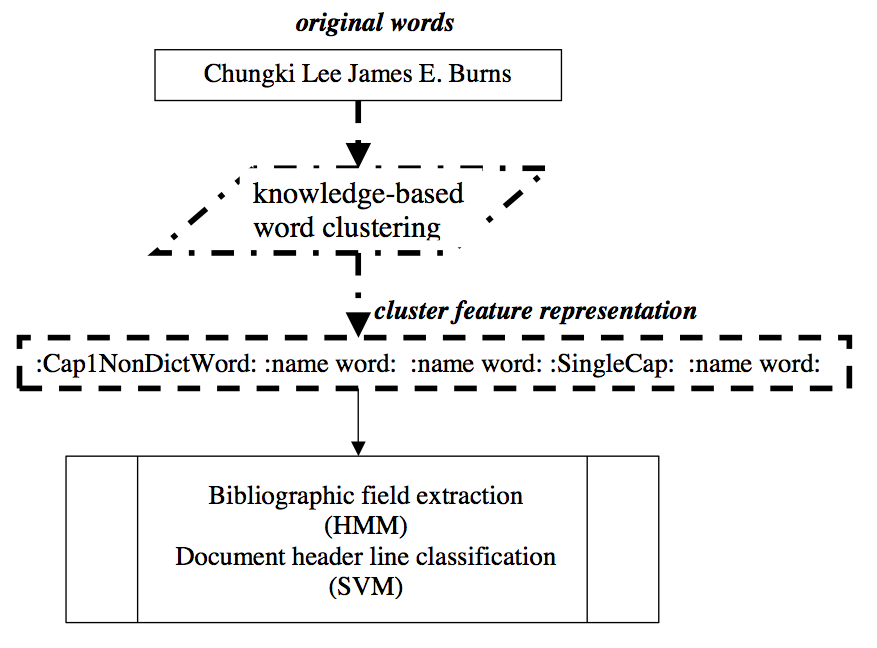
\includegraphics[width=0.7\linewidth]{./assets/workflow-rule-based}
\end{figure}

Han et al. ainda utiliza da técnica  de SVM (Support Vector Machines) para classificação de linhas de um cabeçalho de um documento, tanto em função dos bons resultados obtidos quanto também pela boa performance apresentada. Deste modo, cada linha obtida se transforma em um vetor de palavras, que é comparado com o \textit{cluster}, identificando mais facilmente os metadados.

Além disso é utilizada também a técnica de HMM \cite{Rabiner-HMM-Speech} para a extração das referências, observando sempre a ocorrência de padrões como título e autor para identificação dos mesmos em referências existentes no documento.

Basicamente a \textit{Rule-based Word Clustering} se resume em 3 (três) etapas. A primeira etapa se resume na construção das bases de dados, assim como \cite{Han-SVM}, onde foram utilizadas também como bases externas os nomes apresentados em seu \textit{cluster} de maneira a unir não somente estas bases externas mas também bases construídas dentro de um domínio específico, como palavras que fazem parte de um conjunto finito, não genérico.

A segunda etapa é chamada de \textit{Cluster Design}. Esta etapa é onde os \textit{clusters} são arquitetados, de maneira a contemplar também propriedades ortográficas das palavras, como se funcionasse de maneira geral como uma expressão regular de palavras, formando então um \textit{cluster} com base nas características apresentadas.

A terceira etapa é chamada de \textit{Rule Design}, que resume-se basicamente na representação de cada palavras dentro de seu contexto de apresentação. Por exemplo, nomes devem começar com a primeira letra maiúscula para então serem classificadas como do grupo de ''nomes''.

Como resultado este \textit{cluster} permite um ganho considerável de performance, além de permitir uma precisão maior dos resultados, visto que eles são apresentados com base nestas bases focadas em um domínio específico, perfazendo um contexto mais definido e com resultados mais garantidos ao se comparar por exemplo com técnicas de \textit{cluster} distribuídos.

Por outro lado a utilização desta técnica possui uma falha em semântica dos dados, visto que quando um dígito ou conjunto deles é substituído por \texttt{:number} ele se torna apenas um número, sem um contexto específico, ou seja, pode ser tanto uma referência a alguma página ou até mesmo um mês de um ano.

\subsection{Conditional Random Fields (CRFs)}

% Falar sobre CRFs 

Conditional Random Fields é um framework proposto por Lafferty et al. \cite{crf} criado para construir modelos probabilísticos e dados marcados em sequência (\textit{label sequence data}), geralmente utilizados no reconhecimento de padrões e aprendizado de máquinas (\textit{machine learning}).

Sua representação é puramente matemática com modelos gráficos a fim de maximizar as probabilidades condicionais que se desejam aplicar.

Esta técnica é comparada e quase sempre utilizada juntamente com a HMM (Hidden Markov Models), de maneira a possuir algumas vantagens sobre esta última, como a habilidade de relacionar pressupostos independentes nos modelos, ou seja, relacionar observações e/ou interpretações.

Além disso, CRFs são utilizadas também em marcação e parseamento de dados sequenciais, com uma ordem determinada, como linguagem natural, sequências biológicas (como os genes) ou estados computacionais.

% Falar sobre o uso de CRFs na extração de informação

Sua aplicação na extração de metadados foi apresentada por Peng et al. \cite{crf-ie}, como uma maneira eficaz de extrair padrões em cabeçalhos e referências de artigos científicos. Deste modo, através da identificação destes padrões sequenciais pode-se determinar os tipos de dados existentes e então identificá-los, seguindo uma lógica/ordem pré-determinada.

A utilização de CRFs na extração de metadados mostra-se muito eficaz por reduzir bastante os erros em algumas métricas, aumentando o sucesso da aplicação desta técnica nesta área.













\section{Revisão de Estado da Arte na Extração de Metadados}

\section{Técnicas de Algoritmos}

\section{Ambientes de Extração de Metadados}

% % % % % % % % % %













\section{Trabalhos Comparativos}

\comentario{Falar sobre as comparações realizadas por Granitzer, tanto no que diz respeito a layouts \cite{granitzer-layout-based}, quanto no que diz respeito a dicionários \cite{Granitzer2011a}.}

\section{Ferramentas e Projetos de Destaque}

Alguns projetos baseiam sua extração em padrões pré-definidos de maneira a identificar dados relevantes dentro de uma região específica, facilitando a procura e consequentemente aumentando a velocidade no resultado. 

Estes projetos geralmente permitem uma variedade muito grande de layouts, embora nem todos já estejam previamente definidos. Geralmente novos layouts são inseridos em novas versões ou até mesmo por contribuições das mais diversas, como é o caso dos projetos de código livre, os chamados projetos \textit{open source}.

Abaixo segue uma relação dos principais projetos relacionados à área de extração de metadados de artigos científicos, com informações sobre seu funcionamento e algoritmos que são utilizados.

\subsection{Cermine}

% CERMINE

Um destes projetos é o recente CERMINE \cite{cermine}, uma biblioteca \textit{open source} desenvolvida na linguagem de programação Java que permite que sejam extraídos os metadados de artigos científicos em formato digital PDF, oferecendo ainda a possibilidade de cruzamento de dados por meio de referências e títulos, permitindo assim identificar citações bem como a relevância de um determinado documento.

O CERMINE ainda possui um mecanismo de aprendizagem da própria máquina, permitindo que na medida que dados forem sendo alterados ele consiga absorver os detalhes e permitir assim uma mudança de sua maneira de extrair os dados. Deste modo ele permite que seja adaptado para novos padrões de layouts, o que permite de maneira geral que uma grande gama de modelos seja então abrangida. 

Seu grande diferencial em comparação com as demais técnicas é que ele não somente extrai os metadados de um artigo, mas sim analisa todo o seu conteúdo, incluindo citações a outros artigos, que podem ser facilmente cruzados por meio de informações como título e autor(es).

Seu mecanismo considera somente arquivos PDF com texto gerado de maneira pura, sem a utilização de imagens. Basicamente ele considera regiões, linhas e páginas como pontos estratégicos para a extração de informações. As bases destas regiões possuem padrões que são utilizados juntamente com técnicas de SVM \cite{Han-SVM}. Com base nisso ele condensa um layout onde as informações geralmente estão dispostas, permitindo assim que em um determinado local do arquivo esteja, provavelmente, o título e o nome dos autores. 

Com estas regiões definidas o CERMINE extrai as informações com base em padrões preestabelecidos, de maneira a gerar então sua saída para os metadados e sua saída para as referências encontradas. A saída trabalhada pelo projeto é no formato XML, permitindo assim que possa ser compartilhado com outros sistemas por possuir uma leitura semântica e ao mesmo tempo fácil de ser interpretada pelas linguagens de máquinas. A \autoref{fig:cermine-workflow} demonstra como o processo de extração do CERMINE funciona.

\begin{figure}
\centering
\caption{CERMINE Extraction Workflow}
\label{fig:cermine-workflow}
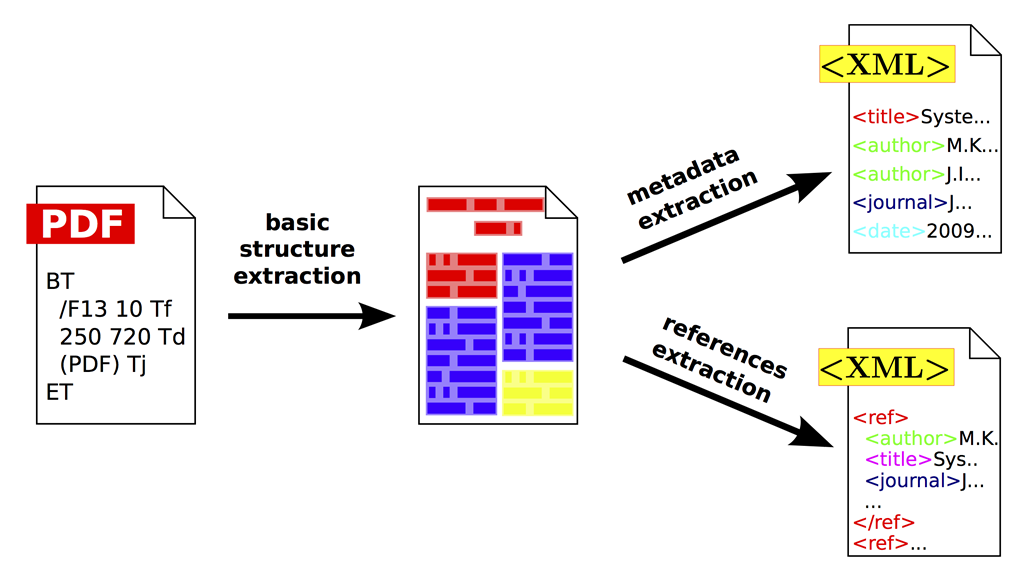
\includegraphics[width=0.7\linewidth]{./assets/cermine}
\end{figure}

Com o mapeamento definido ele identifica regiões de acordo com seu conteúdo, as quais ele chama de \textit{zones}. Esta regiões são determinadas a fim de extrair as informações relevantes para cada uma, de maneira a separar, por exemplo, a área destina aos metadados do arquivo. O CERMINE divide estas \textit{zones} da seguinte maneira:

\begin{itemize}
\item \textbf{Metadata:} É a região mais ao alto do documento, onde obtém os metadados, que seriam o resumo, \textit{bib\_info}, tipo, título, afiliação, autores, datas, editores e palavras-chaves.
\item \textbf{References:} Região responsável por identificas detalhes de referências que foram utilizadas no artigo, como título e autores, por exemplo
\item \textbf{Body:} O texto geral do artigo, incluindo equações, imagens e tabelas.
\item \textbf{Other:} Outros detalhes menos significantes semanticamente, como número das páginas, dentro outros.
\end{itemize}

A extração das referências abrange também seus próprios metadados. Tanto no texto corrido (\textit{Body}) quanto na lista de referências do artigo o \textit{parser} do CERMINE analisa linha a linha, permitindo uma extração de dados mais eficaz. Das referências são extraídos os seguintes dados: autor, título, nome do \textit{journal}, volume, \textit{issue}, páginas, \textit{publisher}, localização e o ano.

\subsection{TeamBeam}

Outros projeto de destaque é o TeamBeam \cite{teambeam}, cuja base ideológica possui objetivos bem sociais, de contribuir com o compartilhamento de conhecimento. Basicamente o objetivo do projeto é extrair metadados de artigos científicos, porém focado apenas nestes, de maneira a extrair título, nome do \textit{journal}, resumo e informações sobre os autores, como nome, endereço de e-mail e afiliações.

O projeto também é de código livre (\textit{open source}) e é baseado na extração de pequenos blocos de texto. A manipulação dos arquivos PDF são feitas pela biblioteca PDFBox \footnote{Biblioteca de manipulação de arquivos PDF mantida pela Fundação Apache. Disponível em \url{https://pdfbox.apache.org/}}, que fornece meios eficazes de extrair textos com base nas regiões desejadas.

O algoritmo do TeamBeam utiliza o algoritmo de \textit{Maximum Entropy} \cite{maximum-entropy}, que utiliza basicamente de tarefas de classificação sequencial como ferramenta principal para obtenção de padrões. A base deste algoritmo está na utilização de CRFs \cite{crf}, principalmente no que diz respeito à extração dos metadados \cite{crf-ie}.

O processo de extração é feito basicamente em duas etapas. A primeira é a etapa de classificação de blocos de texto (\textit{text block classification}), onde geralmente já é possível obter algum dado concreto de resultado. Neste etapa o objetivo é associar certos blocos de texto a um dos seguintes marcadores: \textit{Title Block}; \textit{Sub-Title Block}; \textit{Journal Block}; \textit{Abstract Block}; \textit{Author Block}; \textit{E-Mail Block}; \textit{Affiliation Block}; \textit{Author-Mixed Block}; e \textit{Other Block}.

Dependendo do layout do artigo alguns metadados podem vir divididos em blocos de texto diferentes, necessitando de um processamento posterior, como é o caso, geralmente, dos blocos com informações sobre os autores. Neste caso também é realizada a etapa de classificação de token (\textit{token classification}), que se resume na classificação de palavras individualmente de acordo com um dos seguintes marcadores: \textit{Given Name}; \textit{Middle Name}; \textit{Surname}; \textit{Index}; \textit{Separator}; \textit{E-Mail}; \textit{Affiliation-Start}; \textit{Affiliation}; e \textit{Other}.

Kern et al. defendem a ideia dos excelentes resultados do TeamBeam ao ser comparado com outros projetos. Este fato é dado em virtude das características que são levadas em consideração no processamento do algoritmo, utilizando de dicionários, informações de layout e modelo de linguagem.

\subsubsection{Resultados Comparativos}

A fim de analisar os resultados obtidos com a aplicação das técnicas descritas no TeamBeam, os autores comparam as técnicas utilizadas com outras técnicas de outras ferramentas, que utilizam processos diferentes de análises.

Para fins de comparação de resultados, os autores citam as técnicas ParsCit (\autoref{tec-parscit}), Layout-CRFs (\autoref{tec-layout-crfs}) e Mendeley Desktop (\autoref{tec-mendeley}). Como conclusão ele compara estas três técnicas separadamente, por não abrangerem todos os detalhes que o TeamBeam possui, o que tornaria a comparação desleal.

Assim, ele chega à conclusão que em virtude das diferentes formas de processamento dos dados feitas por cada umas das ferramentas, chega-se a resultados mais precisos para cada campo extraído. Por exemplo, o Layout-CRF's (\autoref{tec-layout-crfs}) é mais abrangente e mais assertivo para extração de títulos, por ser baseado em CRF. Já as ferramentas baseadas em dicionário apresentam melhores resultados para extração de autores, visto se basearem em \textit{data-sets\footnote{Bases de dados com nomes dos autores mais citados e outras informações já catalogadas que são armazenadas para consulta pública.}} já consolidados.

\comentario{Devo explicar aqui o que seriam esses Data-Sets? Exemplo: E-Prints, Mendeley e PubMed.}

\subsection{Layout-CRF's}
\label{tec-layout-crfs}

\comentario{Escrever sobre.}

\subsection{Mendeley Desktop}
\label{tec-mendeley}

\comentario{Escrever sobre.}

\subsection{CiteULike}
\label{tec-citeulike}

\comentario{Escrever sobre CiteULike, com base no artigo de seus autores \cite{citeulike}.}

\subsection{CiteSeer}

Um dos projetos mais específicos encontrados é o CiteSeer \cite{citeseer}. Seu objetivo não é apenas extrair dados em artigos, mas sim também analisar citações de outros documentos no conteúdo textual encontrado. Assim, ele é capaz de identificar quais documentos são citados, quantas vezes são citados e onde são citados, se assemelhando muito ao processo de citação natural.

Desta forma, com estas informações identificadas, ele consegue criar um \textit{ranking} dos documentos citados, incluindo seus autores e \textit{journals}, criando a partir de um documento fonte todo um conjunto de relações com outros documentos de uma maneira estatística bem eficaz.

Os indexes de citações (\textit{citation indexes}), que são utilizados no projeto, foram originalmente criados para a recuperação de informação, porém sua utilidade é tamanha que permite que citações sejam indexadas de maneira eficaz, permitindo inclusive que referências de documentos em idiomas diferentes sejam identificadas. Desta maneira, essa técnica pode ser utilizadas de diversas formas, não somente na identificação de citações propriamente ditas, mas envolvendo um conjunto de informações eficazes, como inclusive identificar a reputação de um determinado artigo científico no meio em que se encontra, simplesmente analisando onde é referência em relação ao número de vezes em que é citado.

Uma proposta interessante em que se baseia o CiteSeer é a de Cameron \cite{cameron}. Seu objetivo é de formar uma Base de Citações Universal, onde todos os artigos estariam ligados entre si, independente de qualquer fator externo como idioma, por exemplo. A diferença entre esta proposta e o trabalho realizado com o CiteSeer é que este último permite que os documentos sejam analisados sem nenhum esforço extra, ou seja, sem a intervenção dos autores dos documentos, como é proposto por Cameron. Neste caso, os documentos seriam analisados de maneira automática, diminuindo o tempo necessário para o relacionamento de todos eles e aumentando a eficácia e eficiência do processo.

O funcionamento do CiteSeer é relativamente simples, porém o trabalho realizado por detrás do processo envolve muito estudo e dedicação. Basicamente ele é capaz de fazer o \textit{download} de \textit{papers} utilizando a Internet, convertê-los em texto e realizar a análise de todas as suas citações. Este resultado é armazenado em um banco de dados para consultas e relacionamentos futuros. Um dos pontos interessantes desta análise é que como ela é feita com base em referência textual, identificado origem e destino, ela pode ser facilmente aplicada tanto no sentido natural de leitura (um artigo cita outros) quanto no sentido inverso (um artigo é citado por outros). 

O projeto também possui suas desvantagens, como por exemplo, a não cobertura de alguns \textit{journals} importantes, indexando todos seus documentos online e de maneira automática. Além disso o projeto original não é capaz de identificar mais de um autor nos documentos, sendo a identificação apenas pelo campo autor, tendo ele apenas um ou mais de um pesquisador envolvido.

Basicamente o projeto analisa o documento em partes:

\begin{itemize}
\item \textbf{URL:} a URL onde o documento foi obtido;
\item \textbf{Cabeçalho:} o bloco de título e autor do documento;
\item \textbf{Resumo:} o bloco de resumo do documento;
\item \textbf{Introdução:} a introdução do texto do documento;
\item \textbf{Citações:} a lista de referências a outros documentos citadas no decorrer do texto;
\item \textbf{Contexto de citação:} o contexto no qual um documento cita outro;
\item \textbf{Texto completo:} o texto completo do documento e suas respectivas citações como um todo.
\end{itemize}

Um dos detalhes importantes do projeto é a identificação das \textit{tags} de citações, que são basicamente as representações visuais quando um outro documento é referenciado, como por exemplo: [4], [Giles997] e ''Marr 1982''. Estes pequenos pedaços de textos que permitem ao CiteSeer identificar a relação (e em que momento do texto) entre documentos, permitindo assim que suas análises sejam realizadas de maneira eficaz.

Uma das dificuldades relatadas durante o desenvolvimento do projeto é a identificação de artigos iguais com formas de escrita e informações divergentes. Alguns artigos podem vir com autores com sobrenomes utilizando abreviação, ou até mesmo em ordem diferente. A fim de aumentar esta identificação alguns passos a mais são realizados, como a conversão para caixa baixa todas as letras, remoção de hifens e das próprias \textit{tags} de citação, expansão de abreviaturas e remoção de algumas palavras externas como ''\textit{volume}'', ''\textit{pages}'' e ''\textit{number}'' por exemplo.

O CiteSeer é um projeto bem maduro e abrangente. Após cerca de 18 (dezoito) anos desde sua criação ele ainda se encontra ativo na Internet, abrangendo cada vez mais documentos e aprimorando cada vez mais suas técnicas de identificação de documentos.

\subsection{ParsCit}
\label{tec-parscit}

Assim como o CiteSeer o ParsCit é um projeto baseado na identificação de citação de documentos. Porém eles utiliza um modelo de CRF \textit{(Conditional Random Fields)} para identificar sequências nas referências. 

O projeto encontra-se ainda ativo e possui atuais contribuições de desenvolvedores ao longo do mundo. Desenvolvido na linguagem de programação \textit{Perl}, o projeto pode ser executado tanto na forma de um \textit{web service\footnote{É a disponibilização de algum serviço na Internet permitindo que outros projetos consultem suas informações e as obtém de maneira simplicada.}} quanto de maneira \textit{standalone}, com execução do código direto quando necessário, dentro do servidor.

Um detalhe bastante interessante do projeto é a descrição de seu processamento antes e depois da análise do documento, que o autor chama de \textit{Pre-Processing Steps} e \textit{Post-Processing Steps}.

Inicialmente o processamento inicia buscando certos \textit{tokens} que podem estar ligados a alguma referência, seja em formato numérico, seja na citação dos nomes dos autores nos mais diversos formatos. Com essa referência coletada o próximo passo é buscar dentro do artigo onde ela está localizada, com base em um conjunto de heurísticas previamente definidas. Para isso é necessária a conversão total do conteúdo do artigo para o formato texto, que deve estar codificado em UTF-8\footnote{Formato de exibição de caracteres que englobam os formatos mais utilizados no mundo, com acentuação e caracteres especiais.}.

Desta forma a fase de pré-processamento se inicia com esta analise puramente textual, em busca de padrões comuns que podem ter sido utilizados para representações de referências à artigos científicos. Com os resultados coletados um modelo CRF é então aplicado aos dados encontrados para processamento futuro.

Com este modelo CRF definido algumas etapas são aplicadas a fim de normalizar os dados encontrados. Nomes de autores podem estar escritos de maneira diferente, com abreviações em nomes de maneira diferente, dependendo do modo como as referências foram escritas no artigo analisado.

Esta análise posterior dos nomes dos autores é feita com base na inspeção de cada palavra individualmente, respeitando então um padrão de normalização definido, sempre com as iniciais dos nomes seguidas do sobrenome escrito normalmente.

A utilização deste projeto é feita de maneira muito simples, podendo ser executado por linha de comando, o que facilitam os testes e a extração de dados. Os resultados obtidos desta análise é então exibido (ou gravado em arquivo) em formato XML, que permite utilização posterior em qualquer tecnologia. Como informado anteriormente os resultados também podem ser coletados em formato de \textit{Web Service}, mas para os fins desta pesquisa apenas sua execução em linha de comando é suficiente.

\subsubsection{Resultados Comparativos}

Visando comparar os resultados obtidos com alguns projetos em que o ParsCit foi baseado, os autores realizam comparações com os resultados obtidos pelo processo descrito por Peng \cite{crf-ie}, onde de maneira geral obteve uma melhora na extração e comparação das referências em torno de 5\% (precisão de 0.91 passou para 0.95), demonstrando a eficácia do projeto.

Visando também analisar outros projetos a mesma comparação de resultados foi feita com o projeto CiteSeer \cite{citeseer}, onde o aumento da qualidade dos dados extraídos foi de aproximadamente 19\% levando em consideração algumas limitações do CiteSeer que não são compreendidas como no ParsCit.

% Falar de cada trabalho encontrado com base nos eventos

	% Falar um resumo
	% Diferencial do projeto
	% Se está ativo ou não
	
\comentario{Seria necessário falar também do Weka (\textit{The open-source machine learning framework})? Até que ponto ele seria relevante para a pesquisa em si? Neste caso tenho medo de fugir muito do escopo e detalhar demais técnicas.}